
\section{Ponteiros}

\begin{frame}[allowframebreaks=0.7]

\frametitle{\Large Capítulo 01 -- Ponteiros}
\begin{columns}
\begin{column}{.4\textwidth}
\centering
Pontos fundamentais a serem cobertos:
  
  \begin{small}
  \begin{enumerate}
  \item \textbf{\textcolor{red}{Pré-requisito: prática na linguagem C}}
  \item Exemplos -- lúdicos
  \item Ponteiros aos diversos tipos de dados
  \item Uso de Memória
%  \item Alocação dinâmica de memória
  \item Alocação de memória Estática x Dinâmica
  \item  Funções para alocação de memória
  \item  Utilizando as funções para alocação de memória
  \item  Alocação de memória e estruturas em C
  \item  Ponteiros para ponteiros
  \item Mais alocação de vetores e matrizes como ponteiros
\end{enumerate}  
  \end{small}
  
\end{column}

\begin{column}{.6\textwidth}
%\centering
%\vspace{-2cm}
\vskip -1.5cm

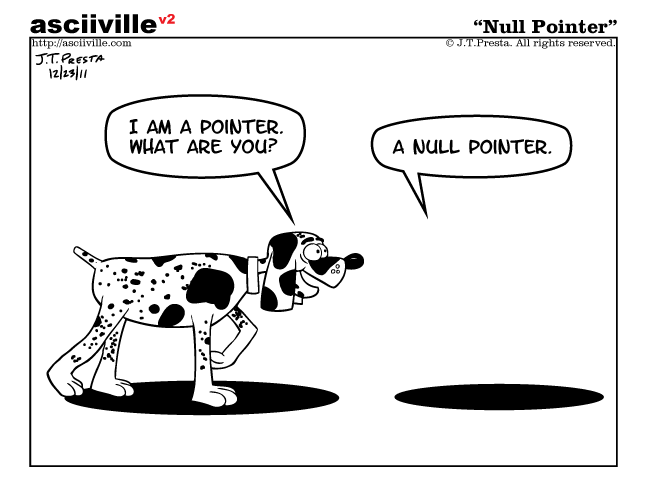
\includegraphics[height=6cm, width=7cm]{figs/fig_ponteiros/nulo-pointer.png}
%\hspace{+0.25cm}
%\scriptsize\textcolor{red}{[Tizio, Caio et al., Nature (2006)]}
\end{column}

\end{columns}

\end{frame}



\begin{frame}[allowframebreaks=0.9]

\frametitle{Motivação aos Ponteiros}
\begin{figure}[ht]
  \begin{center}

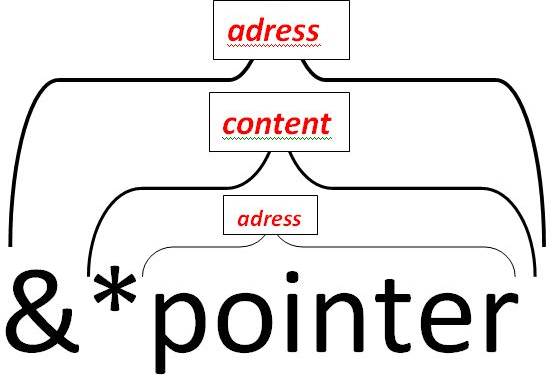
\includegraphics[height=5cm, width=5cm]{figs/fig_ponteiros/hierarq_pointer.png}

    \caption{A história está por vir ...}
 %   \label{fig:}
  \end{center}
\end{figure}

\end{frame}

%------------

%\begin{frame}[c,fragile,plain]{Observem o seguinte código}
\begin{frame}[c,fragile,plain]{Exemplos Lúdicos}

\lstinputlisting{../codes/ponteiros/exemplo01_P.cpp}
\pause

\begin{itemize}
  \item Ao executarmos esse código, qual será a sua saída?
\end{itemize}
\end{frame}



\begin{frame}[c,fragile,plain]{Exemplos e agora?}

\lstinputlisting{../codes/ponteiros/exemplo02_P.cpp}
\pause



\pause
\begin{itemize}
  \item Qual é a saída do código acima? 
% \item Qual(is) é(são) a(s) diferença(s) para o código anterior?
  \item Quando não souber como funciona um comando em C?
  \item Várias respostas ... pense nelas e veja a melhor para voce!
%%%$ man system

\end{itemize}
\end{frame}


\begin{frame}[c,fragile]%[allowframebreaks=0.9]

\frametitle{Reflexões Iniciais sobre Ponteiros}

  \begin{itemize}[<+->]
   \item O operador \& era conhecido 
    \item O operador \texttt{*} (\textbf{estrela} -- afinal é uma estrela em C) era quase desconhecido
    \item Este  último é como um catálogo telefônico, acessa um conteúdo de um assinante via uma página específica
      \item Um ponteiro proporciona um modo de acesso a variáveis sem referenciá-las diretamente
    \item Reflita sobre ponteiros na vida real ... 
  \item Quanto o \texttt{*} é a essência das linguagens C e C++
  \item Entendendo isto vais entender o que há nas bibliotecas, como STL, etc
  \item Resumindo: 
  \pause
  \begin{itemize}
      \item O nome do ponteiro retorna o endereço para o qual ele aponta
      \item O operador (\&) junto ao nome  do ponteiro retorna o endereço do ponteiro
      \item O operador (*) junto ao nome do ponteiro retorna o conteúdo da variável apontada
    \end{itemize}
  \end{itemize}
  
\end{frame}




\subsection{Motivação aos Ponteiros}

\begin{frame}[c]{Ponteiro}

  \begin{itemize}[<+->]
  \item O correto entendimento e uso de ponteiros é crítico para uma programação bem-sucedida em C.
  \item Ponteiros são muitos utilizados em C, em parte porque eles são, às vezes, a única forma de expressar uma computação.
  \item Em alguns casos, o uso de ponteiro resulta em um código mais compacto e eficiente que obtido de outras formas.
  \item Ponteiros e vetores são intimamente, relacionados.  
  \item Aquela parte  de vetores terem dimensões especificadas e fixas, é conhecida como
 \textbf{alocação estática}.
  \item Os ponteiros irão servir para contornar esta limitação
  \end{itemize}
  
\end{frame}

\begin{frame}[c]{Ponteiro}
 \begin{itemize}[<+->]
   \item Basicamente há três razões para utilizar ponteiros:
      \begin{enumerate}[<+->]
        \item Ponteiros fornecem os meios pelos quais as funções podem modificar seus argumentos;
        \item Ponteiros são usados para suportar as rotinas de \textbf{alocação dinâmica} em C;
        \item O uso de ponteiros pode aumentar a eficiência de certas rotinas.
    \end{enumerate}
  \item Por outro lado, ponteiros podem ser comparados ao uso do comando \textbf{goto}, como uma forma diferente de escrever códigos impossíveis de entender. 
 \end{itemize}
\end{frame}

\begin{frame}[c]{Ponteiros e endereços}
  \begin{itemize}[<+->]
    \item Em um máquina típica, a memória é organizada como um vetor de células consecutivas numeradas ou endereçadas, 
    que podem ser manipuladas individualmente ou em grupos contínuos.
  \item Uma situação comum é que qualquer \textit{byte} pode ser um \textit{char}, um par de 
  células de um \textit{byte} pode ser tratado como um inteiro short, etc.
  \item Um ponteiro é um grupo de células que podem conter um endereço.
  
  \begin{figure}[!ht]
     \centering
     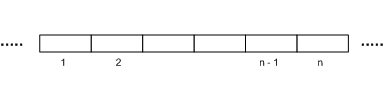
\includegraphics[width=.5\textwidth]{figs/fig_ponteiros/representacao-memoria}  
     \caption{Representação da memória de uma máquina típica} 
  \end{figure}
  \end{itemize}
\end{frame}

\begin{frame}[plain]{Ponteiro}
  \begin{block}{Definição}
     \begin{itemize}[<+->]
        \item É uma \textbf{variável que contém um endereço de memória}. Esse endereço é normalmente a posição de memória de
         uma outra variável.
        \item Se uma variável contém o endereço de uma outra, então a primeira é dita um ponteiro para a segunda.
        \begin{figure}[!htpb]
          \centering
          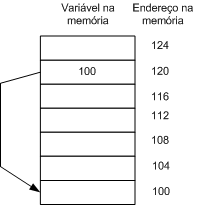
\includegraphics[width=.3\textwidth]{figs/fig_ponteiros/exemplo-representacao-ponteiro}  
           \caption{Representação de ponteiro}    
        \end{figure}
      \end{itemize}
  \end{block}  
\end{frame}

\begin{frame}[c]{Variáveis Ponteiros}
  \begin{enumerate}[<+->]
  \item A linguagem C permite o armazenamento e a manipulação de valores de endereço de memória.
  \item Para cada tipo existente (\texttt{int  long float double  char}), há um tipo ponteiro capaz de armazenar endereços de memória em que existem valores do tipo correspondente armazenados.
  \item Um ponteiro proporciona um modo de acesso a variáveis sem referenciá-las diretamente. 
  \end{enumerate} 
\end{frame}

\begin{frame}[c]{Algumas das razões para utilizar ponteiros são:}
\begin{enumerate}[<+->]
  \item Ponteiros fornecem maneiras com as quais as funções podem realmente modificar os argumentos que recebem.
  \item Para criar estruturas de dados complexas, como listas encadeadas e árvores binárias, onde uma estrutura de dados deve conter referências sobre outra.
  \item Para comunicar informações sobre a memória, como na função \textbf{malloc} que retorna a localização de memória livre através do uso de ponteiro.
  \item Notações de ponteiros compilam mais rapidamente tornando o código mais eficiente.
  \item Para manipular matrizes mais facilmente através de movimentação de ponteiros para elas (ou parte delas), em vez de a própria matriz.
\end{enumerate}
\end{frame}


\begin{frame}[fragile,c]{Variáveis do Tipos de Ponteiros}
  \begin{itemize}[<+->]
    \item A linguagem C não reserva uma palavra especial para a declaração de ponteiros.
    \item As variáveis do tipo ponteiro são declaradas da seguinte forma: \textit{tipo} com os nomes das variáveis precedidos pelo caractere~\textbf{*}.    
    \begin{lstlisting}[language=C]
    int *a, *b; 
        \end{lstlisting}
    \item A instrução acima declara que \textbf{*a} e \textbf{*b} são do tipo \textbf{int} e que \textbf{*a} e \textbf{*b} são ponteiros, isto é \textbf{a} e \textbf{b} contém endereços de variáveis do tipo~\textbf{int}.
  \end{itemize}
\end{frame}

\begin{frame}[fragile,c]{Operadores de Ponteiros}
  \begin{itemize}
    \item A linguagem C oferece dois operadores unários para trabalharem com ponteiros.
  \end{itemize}
  \begin{table}
     \begin{tabular}{c|c}
     \hline Operador & significado\\
      \hline \& & (``endereço de'')\\      
      \hline * & (``conteúdo de'')\\
      \hline 
     \end{tabular}
  \end{table}   
\end{frame}

\begin{frame}[fragile,c]{Operadores de Ponteiros}
  \begin{itemize}[<+->]
     \item O operador \& (``endereço de''), aplicado a variáveis, resulta no \alert{endereço da posição da memória} reservada para a variável. Por exemplo,
     \begin{lstlisting}[language=C]
       a = &b;     
     \end{lstlisting}
      \item coloca em \textbf{a} o endereço da memória que contém a variável \textbf{b}.
    \item O endereço não tem relação algum com o valor da variável \textbf{b}.    
      \item Após as declarações as duas variáveis armazenam  ``lixos'', pois não foram inicializadas.
 \end{itemize}  
\end{frame}

\begin{frame}[fragile,c]{Operadores de Ponteiros}
  \begin{itemize}[<+->]
    \item O operador * (``conteúdo de''), aplicado a variáveis do \alert{tipo ponteiro}, acessa o \alert{conteúdo do endereço da memória} pela variável ponteiro, isto é, devolve o conteúdo da variável apontada pelo operando. Por exemplo:
    \begin{lstlisting}[language=C]
       a = *b;
    \end{lstlisting}
    \item Coloca o valor de \textbf{b} em \textbf{a}, ou seja, \textbf{a} recebe o valor que está no endereço \textbf{b}.
  \end{itemize}
\end{frame}

\begin{frame}[fragile,c]{Atribuição e acessos de endereço}
 \begin{lstlisting}[language=C]
   /* a recebe o valor 5*/
   a = 5;
   
   /* p recebe o endereco de a (p aponta para a). */
    p = &a;
    
    /* conteudo de p recebe o valor 10 */
    *p = 10;
 \end{lstlisting}
\end{frame}

\begin{frame}[plain,c]{Atribuição e acessos de endereço}  
    \begin{columns}
    \column{5cm}
      \begin{figure}[ht]
        \centering
        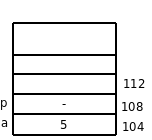
\includegraphics[width=.6\textwidth]{figs/fig_ponteiros/memoria-atribuicao-a}
      \end{figure}
    \column{5cm}
        \begin{figure}[ht]
          \centering
          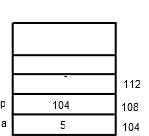
\includegraphics[width=.6\textwidth]{figs/fig_ponteiros/memoria-atribuicao-p}
        \end{figure} 
    \end{columns}
    \begin{figure}[ht]
          \centering
          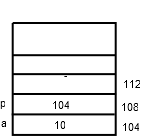
\includegraphics[width=.4\textwidth]{figs/fig_ponteiros/memoria-atribuicao-pa}
          \caption{Efeito da atribuição de variáveis na pilha de execução}
    \end{figure}
\end{frame}

\begin{frame}[fragile,plain,c]{Atribuição de Ponteiros}
  \begin{itemize}[<+->]
    \item Assim como ocorre com qualquer variável,
     também podemos atribuir um valor a um ponteiro. Exemplo:
  \end{itemize}
  
  \begin{minipage}[b]{0.45\linewidth}
  \begin{lstlisting}[language=C]
  void main(void) {
    int a = 10;
    int *b, *c;
    b = &a;
    c = b;
    printf("%p", c);
  }
  \end{lstlisting}
  \end{minipage}
  \hspace{0.1cm}
  \begin{minipage}[b]{0.45\linewidth}
      \begin{figure}[!ht]
       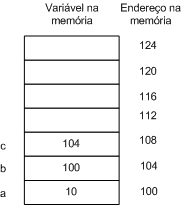
\includegraphics[width=.6\columnwidth]{figs/fig_ponteiros/exemplo-atribuicao-ponteiro}
       % \caption{Exemplo de atribuição valores a Ponteiros}
      \end{figure}
    \end{minipage}  
\end{frame}

\begin{frame}[fragile,c]{Operações com Ponteiros}  
  \begin{itemize}[<+->]
    \item \textbf{Incremento/Decremento}:
    \begin{itemize}[<+->]
      \item Podemos incrementar um ponteiro através da adição regular ou pelo operador de incremento (++).
      \item Incrementar um ponteiro implica na movimentação do mesmo para o próximo tipo apontado.
     
      \item Se \textbf{pa} é um ponteiro para inteiro tem no seu conteúdo o valor 200 (um endereço), depois de executada a instrução, \textbf{pa++}, o valor de \textbf{pa} será o endereço 204 (compiladores onde um inteiro é 4 bytes) e não 201.
     
      \item \textcolor{red}{Logo, cuidar com o compilador e arquitetura em questão: 16, 32, 64 ou 128 bits}
    
      \item Com isso, cada vez que incrementamos \textbf{pa} ele apontará para o próximo tipo apontado.
      \item O mesmo é verdadeiro para o operador de decremento (- -)
      \item Cuidar ainda: associatividade  (esq $\Leftrightarrow$ dir) e precedência (ver manual da linguagem) $\Rightarrow$ fazer os exercícios e ir anotando as respostas
    \end{itemize}
  \end{itemize}
\end{frame}

\begin{frame}[fragile,c]{Operações com Ponteiros}  
  \begin{itemize}[<+->]
    \item \textbf{Comparações entre Ponteiros}:
    \begin{itemize}[<+->]
      \item Ponteiros podem ser comparados:
\begin{lstlisting}[language=C]
  if (pa <> pb)
\end{lstlisting}
      \item Testes relacionais com $>=, <=, >, <$ são aceitos entre ponteiros, desde que os operandos sejam ponteiros.
      \item \alert{O tipo dos operandos devem ser o mesmo, para não obter resultados sem sentido}.
      \item Variáveis ponteiros podem ser testadas quanto à igualdade (==) ou desigualdade(!=) onde os operandos são ponteiros, ou um dos operandos NULL.
    \end{itemize}
  \end{itemize}
\end{frame}

\begin{frame}[fragile,c]{Operações com Ponteiros}
\begin{itemize}[<+->]
  \item \textbf{Atribuição}:
  \begin{itemize}[<+->]
    \item Um endereço pode ser atribuído a um ponteiro através do operador unário \& junto a uma variável simples. Exemplo: 
\begin{lstlisting}[language=C]
  pa = &a;
\end{lstlisting}
  \end{itemize}
  \item \textbf{Leitura de valores}:
  \begin{itemize}[<+->]
    \item O operador (*) devolve o valor guardado no endereço apontado.
  \end{itemize}
  \item \textbf{Leitura do endereço do ponteiro}:
  \begin{itemize}[<+->]
    \item Os ponteiros variáveis também têm um endereço e um valor.
    \item O operador (\&) retorna a posição da memória onde o ponteiro está localizado. Em resumo:        
    \begin{enumerate}[<+->]
      \item O nome do ponteiro retorna o endereço para o qual ele aponta.
      \item O operador (\&) junto ao nome  do ponteiro retorna o endereço do ponteiro.
      \item O operador (*) junto ao nome do ponteiro retorna o conteúdo da variável apontada. 
    \end{enumerate}
  \end{itemize}
\end{itemize}
\end{frame}

\begin{frame}[c]{Chamadas por valor  $\times$ referência}  
  \begin{itemize}
    \item A passagem de argumentos para funções em C são feitas por valor (``chamada por valor'').
    \item Na passagem de parâmetro por valor a função chamada \alert{não pode alterar} uma variável da função que fez a chamada.
    \item Sim, a chamada por valor cópia protege  o conteúdo
    \item Mas, muitas vezes a duplicação do valor da variável deve ser evitado, ai precisamos
    da chamada por referência.
    \item Uso de ponteiros
  \end{itemize}
\end{frame}

\begin{frame}[plain,c]{Atribuição e acessos de endereço}  
  \begin{figure}[!htpb]
      \centering
      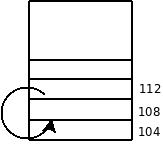
\includegraphics[width=.4\textwidth]{figs/fig_ponteiros/representacao_grafica_valor_ponteiro}
      \caption{Representação gráfica do valor de um ponteiro}
  \end{figure}
\end{frame}

\begin{frame}[fragile,c]{Chamada por referência}
\begin{lstlisting}[language=C]
/*Ordena o vetor v de tamanho n, v[0 .. n-1] 
 * em ordem crescente.
 */
void ordenacaoSelecao(int n, int v[]){
 int i, j;
 for(i = 0; i < n -1; i++)
   for(j = i + 1; j < n; j++)
     if (v[j] < v [i])
       troca(v[i],v[j]); 
}

void troca(int x, int y) {
  int tmp =x;
  x = y;
  y = tmp;
}
\end{lstlisting}
\end{frame}

\begin{frame}[c]{Chamada por referência}
  \begin{itemize}[<+->]
    \item O código anterior cumpre o seu objetivo?
    \item Por causa da chamada por valor, a função \textbf{troca} não afeta os argumentos \textbf{x} e \textbf{y} da rotina que chama, ou seja, o código está \alert{ERRADO}.
    \item Para obter o efeito desejado é necessário passar os endereços dos valores a serem permutados:   
    \begin{itemize}
      \item \textbf{troca}(\&v[i], \&v[j]); 
    \end{itemize}
    \item O que muda na função troca?
  \end{itemize}
\end{frame}

\begin{frame}[fragile,plain,c]{Chamada por referência}
\begin{lstlisting}[language=C]
/* Ordena o vetor v de tamanho n, v[0 .. n-1] 
 * em ordem crescente.
 */
void ordenacaoSelecao(int n, int v[]){
 int i, j;
 for(i = 0; i < n -1; i++)
   for(j = i + 1; j < n; j++)
     if (v[j] < v [i])
       troca(&v[i],&v[j]); 
}
/*Permuta x e y*/
void troca(int *x, int *y) {
  int tmp = *x;
  *x = *y; 
  *y = tmp;
}
\end{lstlisting}
\end{frame}

\begin{frame}[c]{Passagem por referência}
\begin{itemize}
  \item No código anterior os argumentos da função \textbf{troca} foram declarados como ponteiros.
  \item Os parâmetros ponteiros da função \textbf{troca} são ditos como de \textbf{entrada} e \textbf{saída}. 
  \item Dessa forma, qualquer modificação realizada em \textbf{troca} fica visível à função que chamou.
  \item \alert{Para que uma função gere o efeito de chamada por referência, os ponteiros devem ser utilizados na declaração dos argumentos e a função chamadora deve mandar endereços como argumentos}.
\end{itemize}
\end{frame}

\section{Ponteiros e Matrizes}
\begin{frame}[c]{Ponteiros e matrizes}  
  \begin{itemize}[<+->]
    \item Em C, há um estreito relacionamento entre ponteiros e matrizes.
    \item O compilador transforma matrizes em ponteiros após a compilação do código.
    \item Qualquer operação que possa ser feita com índices de uma matriz pode ser feita com ponteiros.
    \item O nome de uma matriz é um endereço, ou seja, um ponteiro.
    \item Ponteiros e matrizes são idênticos na maneira de acessar a memória.
    \item Um \textbf{ponteiro variável} é um endereço onde é armazenado um outro endereço.
  \end{itemize}
\end{frame}

\begin{frame}[fragile,plain,c]{Exemplos de programas com matrizes}


\lstinputlisting{../codes/ponteiros/exemplo03_P.cpp}
\pause
\textcolor{red}{Vários elementos neste código}

\end{frame}


\begin{frame}[fragile,plain,c]{Exemplos de programas com matrizes}


\lstinputlisting{../codes/ponteiros/exemplo04_P.cpp}
\pause
\textcolor{red}{Pergunta de aluno do  laboratório}

\end{frame}



\begin{frame}[fragile,plain,c]{Exemplos de programas com matrizes}

\lstinputlisting{../codes/ponteiros/exemplo05_P.cpp}
\textcolor{red}{Dúvida de aula ... qual a saída do código acima?}

\pause

\begin{lstlisting}[language=C]
[ccs@gerzat ponteiros]$ ./a.out 
9 8 7 99 88 77 1 2 3 
 ... Acabou ....
\end{lstlisting}

\end{frame}





\begin{frame}[fragile,plain,c]{Exemplo de programas com matrizes}
\begin{lstlisting}[language=C]
/*imprime os valores da matriz*/
main(){
   int nums [5] = {100,200,90,20,10};
   int d;
   for(d = 0; d < 5; d++)
   printf("%d\n", nums[d]);
}

/*usa ponteiros para imprimir os valores da matriz*/
main(){
   int nums [5] = {100,200,90,20,10};
   int d;
   for(d = 0; d < 5; d++)
     printf("%d\n", *(nums + d));
}
\end{lstlisting}
\end{frame}

\begin{frame}[fragile,plain,c]{Ponteiros e matrizes}  
  \begin{itemize}[<+->]
    \item O segundo programa é idêntico ao primeiro, exceto pela expressão \textbf{*(nums + d)}.
    \item \alert{O efeito de \textbf{*(nums + d)} é o mesmo que \textbf{nums[d]}}.
    \item A expressão \textbf{*(nums + d)} é o endereço do elemento de índice \textbf{d} da matriz.
    \item Se cada elemento da matriz é um inteiro e d = 3, então serão pulados 6 bytes para atingir o elemento de índice 3.
    \item Assim, a expressão \textbf{*(nums + d)} não significa avançar 3 \textit{bytes}, além \textit{nums} e sim 3 elementos da matriz.
  \end{itemize}
\end{frame}




\begin{frame}[fragile,plain,c]{Cuidados}  

\begin{verbatim}

int vetor[10];
int *ponteiro, i;
ponteiro = &i;

/* as operacoes a seguir sao invalidas */
vetor = vetor + 2; /* ERRADO: vetor nao eh variavel */
vetor++;           /* ERRADO: vetor nao eh variavel */
vetor = ponteiro;  /* ERRADO: vetor nao eh variavel */

/* as operacoes abaixo sao validas */

ponteiro = vetor;   /* CERTO: ponteiro eh variavel */
ponteiro = vetor+2; /* CERTO: ponteiro eh variavel */
\end{verbatim}


\end{frame}


\subsection{Indireção Múltipla}
\begin{frame}[c]{Indireção múltipla}
\begin{block}{O que é \textit{indireção} múltipla?}
  \begin{itemize}[<+->]
    \item \textit{Indireção múltipla} ou \textbf{ponteiro de ponteiros} é quando temos um ponteiro apontando para outro ponteiro que aponta para o valor final.
    \item O valor normal de um ponteiro é o endereço de uma variável que contém o valor desejado.
    \item No caso de um ponteiro para um ponteiro, o primeiro contém o endereço do segundo que aponta para a variável que contém o valor desejado.
    \item A \textit{indireção múltipla} pode ser levada a qualquer dimensão desejada. 
  \end{itemize}
\end{block}    
\end{frame}

\begin{frame}[c]{Indireção múltipla}
  \begin{figure}[ht]
    \centering
    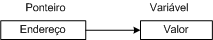
\includegraphics[width=.6\textwidth]{figs/fig_ponteiros/indirecao-simples} 
    \caption{Indireção simples}
  \end{figure}
            
  \begin{figure}[ht]
    \centering
    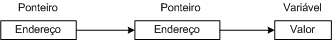
\includegraphics[width=.6\textwidth]{figs/fig_ponteiros/indirecao-multipla}
    \caption{Indireção múltipla}
  \end{figure}
\end{frame}

\begin{frame}[fragile,c]{Indireção múltipla}
\begin{block}{Declaração}
  \begin{itemize}[<+->]
    \item Uma variável que é um ponteiro para um ponteiro deve ser declarada como tal.
    \item A declaração de ponteiro de ponteiro é realizada colocando-se um \textbf{*} adicional na frente do nome da variável. Exemplo:   
\begin{lstlisting}
int **a;
float **b;
\end{lstlisting}
  \item No primeiro exemplo, temos a declaração de um ponteiro para um ponteiro de inteiro (\textbf{int}). 
  \item \alert{É importante salientar que \textbf{a} não é um ponteiro para um número inteiro, mas um ponteiro para um ponteiro inteiro.}
  \end{itemize}
\end{block}    
\end{frame}

\begin{frame}[fragile,c]{Exemplo de indireção múltipla}
\begin{lstlisting}[language=C]
int main(void) {
  int x, *a, **b;
  x = 4;
  a = &x;
  b = &a;
  printf("%d ", **b);
}
\end{lstlisting}
\end{frame}


\section{Ponteiro para Funções}
\begin{frame}[fragile,c]{Ponteiro para funções}
  \begin{itemize}[<+->]
    \item Um recurso muito poderoso da linguagem C, é o ponteiro para função.
    \item Embora uma função não seja uma variável, ela tem uma posição física na memória que pode ser atribuída a um ponteiro. Exemplo:
\begin{lstlisting}[language=C]
int main(){
  int (*func)(const char*, ...);
  func = printf;
  (*func)("%d\n", 1);
}
\end{lstlisting}
 \item No código acima, a instrução
\begin{lstlisting}[language=C]
 int (*func)(const char*, ...);
\end{lstlisting} 
declara uma função do tipo \textbf{int}. Nesse exemplo, estamos declarando que \textbf{func} é uma função do tipo ponteiro para inteiro que aponta para o endereço da função \textit{printf}, através da instrução: 
\begin{lstlisting}[language=C]
 func = printf;
\end{lstlisting}
\end{itemize}
\end{frame}

\begin{frame}[fragile,c]{Ponteiro para funções}
\begin{itemize}[<+->]
  \item A declaração anterior é possível e válida, porque quando compilamos uma função, o código-fonte é transformado em código-objeto e um ponto de entrada é estabelecido. 
  \item Quando é feita uma chamada à função, enquanto o programa está sendo executado, é efetuado uma chamada em linguagem de máquina para esse ponto de entrada.
  \item Portanto, se um ponteiro contém o endereço do ponto de entrada de uma função, então ele pode ser usado para chamar essa função.
  \item Dessa forma, ao executarmos a instrução:
\begin{lstlisting}[language=C]
(*func)("\%d\n", 1);
\end{lstlisting} estamos executando a função \textbf{printf}, logo, será apresentado na saída, o valor 1.
\end{itemize}
\end{frame}

\begin{frame}[fragile,c]{Ponteiro para funções}
\begin{itemize}[<+->]
  \item O endereço de uma função é obtido usando o nome da função sem parênteses ou argumentos. 
  \item Observe que não colocamos parênteses junto ao nome da função. Se eles estiverem presentes como em:  
\begin{lstlisting}[language=C]
func = printf();
\end{lstlisting}, estaríamos atribuindo a \textit{\textbf{func}} o valor retornado pela função e não o endereço dela.
  \item \alert{O nome de uma função desacompanhado de parênteses é o endereço dela.}  
\end{itemize}
\end{frame}

%\imageframe{question}

\begin{frame}[fragile,c]{Ponteiro para funções}  
  \begin{itemize}[<+->]
    \item Nesse exemplo,nada é obtido e bastante confusão é introduzida. Porém, há momentos em que é vantajoso passar funções arbitrárias para procedimentos, ou manter uma matriz de funções.
    \item Por exemplo, escolher o melhor algoritmo para resolver um problema.
  \end{itemize}
\end{frame}

\begin{frame}[fragile,c]{Ponteiro para funções}  
\begin{lstlisting}[language=C]
/**
 * Ordena o vetor v de tamanho n, utilizando 
 * o algoritmo de ordenacao implementado pela 
 * funcao: algOrdenacao.
 */
void ordenar(int v[], int n, 
   void (*algOrdenacao)(int v[], int n)){   
   (*algOrdenacao)(v,n);     
}
\end{lstlisting}  
\end{frame}

\begin{frame}[fragile,c]{Ponteiro para funções}  
\begin{itemize}
  \item Em resumo podemos:  
    \begin{enumerate}
      \item Declarar um ponteiro para uma função.
      \item Atribuir o endereço de uma função a um ponteiro.
      \item Chamar a função através do ponteiro para ela.
    \end{enumerate}
  \item Mas não podemos:  
    \begin{enumerate}
      \item Incrementar ou decrementar ponteiros para funções.
      \item Incrementar ou decrementar nomes de funções.
    \end{enumerate} 
\end{itemize}
\end{frame}


\section{Alocação dinâmica}
\begin{frame}[c]{Alocação dinâmica}
  \begin{itemize}[<+->]
    \item Na declaração de um vetor visto até agora é necessário conhecer e informar o número de elementos do vetor.
    \item Esse pré-dimensionamento é um fator limitante, pois, nos obriga a conhecer de antemão a quantidade de elementos do vetor.
    \item Uma solução é dimensionar o vetor com um número muito alto, para não termos limitações no momento de utilização do programa.
    \item Essa solução leva a um desperdício de memória.
    \item Qual a solução?   
    \begin{itemize}[<+->]
      \item Utilizar alocação dinâmica.
      \item Isto é, requisitar espaços de memória em tempo de execução.
    \end{itemize}
  \end{itemize}
\end{frame}

\begin{frame}[plain,c]{Uso da memória}  
  % \begin{itemize}
  %   \item De modo geral, podemos dizer que existem três maneiras de reservar espaços de memória para o armazenamento de informações, conforme ilustra a figura abaixo.
  % \end{itemize}
  \begin{figure}[ht]
      \centering
      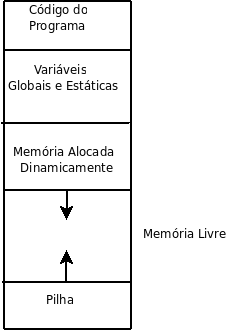
\includegraphics[width=.4\textwidth]{alocacao_esquematica_memoria}
  \end{figure}
\end{frame}

\begin{frame}[fragile,plain,c]{Funções para alocação dinâmica de memória}
  \begin{itemize}[<+->]
    \item A função básica para alocar memória é \textbf{malloc}.
    \item A função \textbf{malloc} recebe como parâmetro o número de \textit{bytes} que se deseja alocar e retorna o endereço inicial da área de memória alocada. 
    \item O código seguinte realiza a alocação dinâmica de um vetor de inteiros com 10 elementos.
\begin{lstlisting}[language=C]
  int *v;
  v = malloc(10*4);
\end{lstlisting}
      \item Após a execução, se a alocação for bem-sucedida, \textbf{v} armazenará o endereço inicial de uma área contínua de memória suficiente para armazenar 10 valores inteiros.
      \item Podemos tratar \textbf{v} como tratamos um vetor declarado estaticamente.
      \item Para ficarmos independente de compilador e máquinas, usamos o operador \textbf{sizeof()}. 
\begin{lstlisting}[language=C]
   int *v;
   v = malloc(10*sizeof(int));
\end{lstlisting}
  \end{itemize}
\end{frame}

\begin{frame}[fragile,plain,c]{Funções para alocação dinâmica de memória}  
  \begin{itemize}[<+->]
  \item A função \textbf{malloc} pode ser utilizada para alocar espaço para armazenar valores de qualquer tipo.
  \item O retorno da função \textbf{malloc} é um ponteiro genérico, para um tipo qualquer, representado por \textbf{void*}, que pode ser convertido para o tipo apropriado da atribuição.
  \item É comum fazer a conversão explicitamente, realizando um \alert{cast} para o tipo correto. Exemplo: 
\begin{lstlisting}[language=C]
 int *v;
 v = (int*) malloc(10 * sizeof(int));
\end{lstlisting}
    \item Se porventura, não houver espaço livre suficiente para realizar a alocação, a função retorna um endereço nulo, representado por \alert{NULL}, definido em \textit{stdlib.h}.
    \item Podemos verificar se a alocação foi realizada adequadamente, testando o retorno da função \textbf{malloc}. Exemplo:
\begin{lstlisting}[language=C]
 v = (int*) malloc(10 * sizeof(int));
 if (v == NULL) 
   printf("Memoria insuficiente.\n");
\end{lstlisting}
\end{itemize}
\end{frame}

\begin{frame}[fragile,c]{Funções para alocação dinâmica de memória}
  \begin{itemize}[<+->]
    \item Para liberar um espaço de memória alocado dinamicamente, usamos a função \textbf{free()}.
    \item A função \textbf{free()} recebe como parâmetro o ponteiro da memória a ser liberado.
\begin{lstlisting}[language=C]
free(v);
\end{lstlisting}
    \item Só podemos passar para a função \textbf{free()} um endereço de memória que tenha sido alocado dinamicamente.
    \item Não podemos acessar o espaço de memória depois de liberado.
  \end{itemize}  
\end{frame}

\begin{frame}[fragile,c]{Funções para alocação dinâmica de memória}
  \begin{table}
   \centering
    \begin{tabular}{p{4cm}p{6cm}}
      \hline \textbf{Função} & \textbf{Descrição} \\
      \hline  \textbf{malloc}(\textit{$<$qtd. bytes$>$}) & Aloca uma área da memória e retorna a referência para o endereço inicial, se existir memória disponível. Caso contrário, retorna \textbf{NULL}.  \\
      \hline \textbf{sizeof}(\textit{$<$tipo$>$})  & Retorna a quantidade de memória necessária para para alocar um determinado tipo.\\
      \hline \textbf{free}(\textit{$<$variável$>$})  & Libera o espaço de memória ocupado por uma variável alocada dinamicamente.\\
      \hline
    \end{tabular}
  \end{table} 
\end{frame}
